\documentclass[aspectratio=169]{beamer}
\usetheme{metropolis}
\usepackage{graphicx}
\usepackage{booktabs}
\usepackage{amsmath}
\usepackage[T1]{fontenc}
\usepackage[utf8]{inputenc}
\graphicspath{{../results/figures/}}

\title{How do alveolar cells fail in lethal COVID-19?}
\subtitle{An ablation-first, replication-audited trajectory analysis}
\author{[Author] --- Systems Biology class presentation}
\date{\today}

\begin{document}
\maketitle

% ---------------------------------------------------------------
\begin{frame}{The question in one sentence}
\Large
Do alveolar epithelial cells in lethal COVID-19 fail as a \alert{coherent block}
(pushed toward one damaged state), or as a \alert{continuous graded collapse}
(spread out in many directions)?
\normalsize
\vspace{1em}
\begin{itemize}
  \item ``Block'' $\Rightarrow$ expect \textbf{centroid displacement}.
  \item ``Collapse'' $\Rightarrow$ expect \textbf{dispersion / variance inflation}.
  \item These predict opposite things, so the failing test is informative.
\end{itemize}
\end{frame}

% ---------------------------------------------------------------
\begin{frame}{Why this matters (and why I'm not claiming new biology)}
\begin{itemize}
  \item Melms 2021, Delorey 2021, Bharat 2020 already described alveolar
        injury in COVID-19 lungs.
  \item My contribution is \textbf{methodological}: a pre-registered,
        ablation-first, replication-audited trajectory pipeline.
  \item Three pre-registered criteria, each with a null and a test statistic,
        declared \emph{before} I looked at the numbers.
\end{itemize}
\end{frame}

% ---------------------------------------------------------------
\begin{frame}{Data}
\begin{itemize}
  \item \textbf{Primary}: SCP1219 (Melms 2021) --- 116{,}313 snRNA-seq nuclei,
        22{,}128 AT1/AT2/ECM-high, 7 healthy + 20 COVID-19 donors.
  \item \textbf{Replication}: cellxgene census (HLCA-extended + Krasnow),
        \emph{SCP1219 removed by \texttt{dataset\_id}}. 89{,}736 AT1/AT2 cells,
        618 donors, 35 datasets.
  \item Primary has full transcriptome; replication has a curated 84-gene
        panel (enough to score programs, too narrow for a new manifold).
\end{itemize}
\end{frame}

% ---------------------------------------------------------------
\begin{frame}{Pipeline at a glance}
\begin{itemize}
  \item Scanpy 1.12.1, harmonypy 0.2.0, Python 3.12.3, seed 42.
  \item Normalize $\to$ log1p $\to$ 3{,}000 HVGs $\to$ 50-PC PCA $\to$
        Harmony on \texttt{donor\_id} $\to$ $k$NN ($k{=}15$) $\to$ UMAP,
        diffusion map.
  \item Diffusion pseudotime rooted at the healthy-AT2 centroid, normalized
        to $[0,1]$.
  \item 8 curated gene programs (\texttt{sc.tl.score\_genes} vs \texttt{.raw}).
  \item \textbf{10 pre-specified ablations.}
\end{itemize}
\end{frame}

% ---------------------------------------------------------------
\begin{frame}{The manifold}
\centering
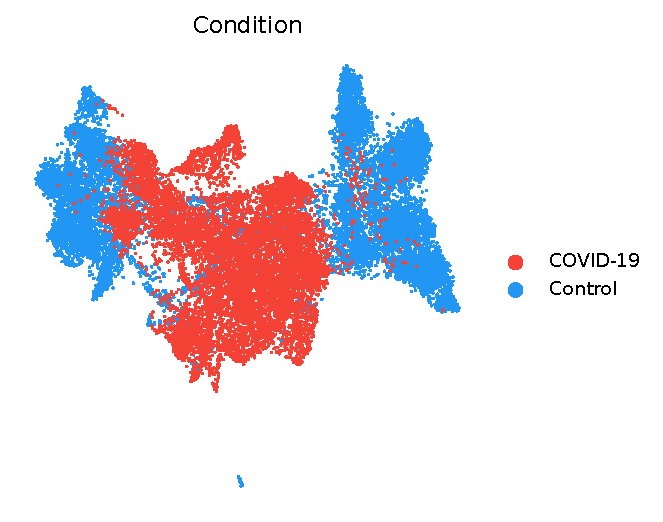
\includegraphics[width=0.45\linewidth]{fig1a_condition.pdf}\hfill
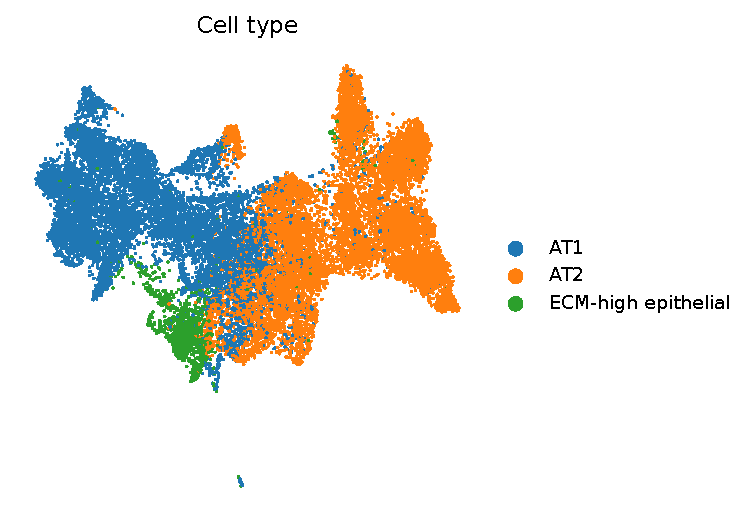
\includegraphics[width=0.45\linewidth]{fig1b_celltype.pdf}
\\
{\small Left: UMAP coloured by condition. Right: by cell type.}
\end{frame}

% ---------------------------------------------------------------
\begin{frame}{Result 1 --- pseudotime shift (supported)}
\begin{itemize}
  \item Control median 0.063; COVID median 0.111; $\Delta = +0.0483$.
  \item 1{,}000-permutation null: $p = 0.001$.
  \item Leave-one-donor-out: direction preserved in \textbf{27/27} donors.
\end{itemize}
\centering
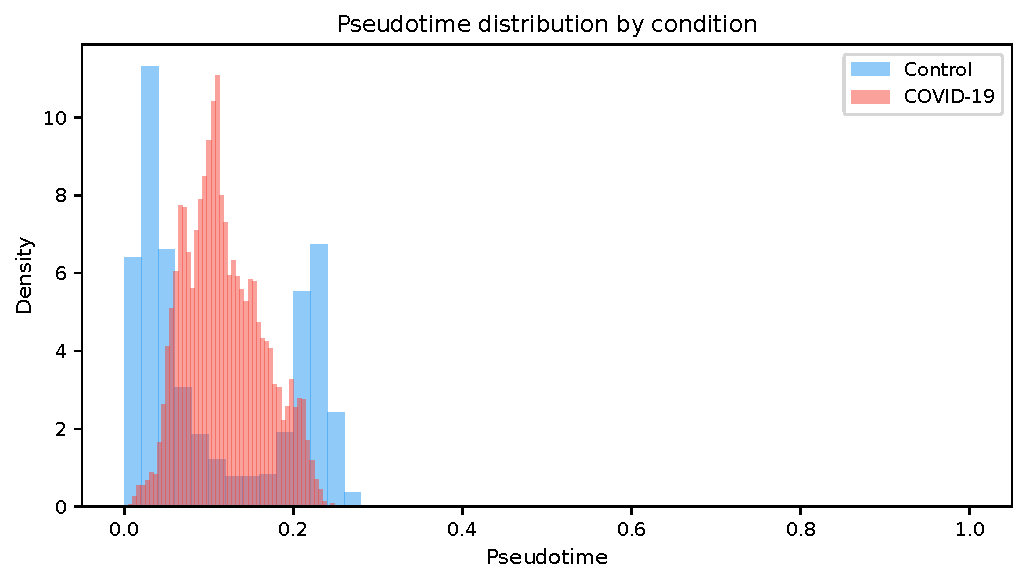
\includegraphics[width=0.55\linewidth]{fig4_pseudotime_density.pdf}
\end{frame}

% ---------------------------------------------------------------
\begin{frame}{Result 2 --- centroid displacement \alert{fails}}
\begin{itemize}
  \item One-sided Mann--Whitney $U$ in PCA-50 (COVID $>$ Healthy): $p = \textbf{1.0}$.
  \item COVID median actually \emph{lower} than healthy.
\end{itemize}
\alert{The ``mono-directional damage'' effect model is wrong.}
This is the most informative finding of the paper: the failure tells you
the effect is \emph{not} a pushed centroid.
\end{frame}

% ---------------------------------------------------------------
\begin{frame}{Result 3 --- dispersion (the real signal)}
\begin{itemize}
  \item Variance in PCA-50 distance to own centroid:\\
        COVID \textbf{33.28} vs.\ Healthy \textbf{14.58} (2.3-fold).
  \item Levene statistic 276.5, $p < 10^{-30}$.
\end{itemize}
\alert{COVID-19 AT1/AT2 cells are \emph{spread out}, not \emph{pushed away}.}
This is the ``robustness collapse'' signature.
\end{frame}

% ---------------------------------------------------------------
\begin{frame}{Ten ablations --- the stress tests}
\scriptsize
\begin{tabular}{lrrr l}
\toprule
Ablation & MPD & $\rho$ & $r$ & Notes \\
\midrule
1 AT2-only              & $+0.133$ & 0.33 & $-0.29$ & sign flip \\
2 UMAP / diffmap        & $+0.048$ & 0.55 & $+0.14$ & unchanged \\
3 Harmony corrected     & $+0.125$ & 0.45 & $+0.14$ & \textbf{amplifies shift} \\
3 Uncorrected           & $+0.048$ & 0.55 & $+0.14$ & baseline \\
4 No apoptosis genes    & $+0.074$ & 0.50 & $+0.14$ & slight up \\
5 4 roots               & $-0.037$ to $+0.048$ & $-0.10$ to 0.64 & $+0.14$ & root-dependent \\
6 Broader epithelial    & $-0.008$ & 0.83 & $+0.25$ & \alert{shift abolished} \\
7 LOO (27 donors)       & 0.028--0.202 & varies & --- & direction 27/27 \\
8 Curated-only          & $+0.048$ & $1.00$ & $+0.14$ & stable \\
8 MSigDB-only           & $+0.048$ & $-0.80$ & $+0.14$ & \alert{ordering inverted} \\
9 Palantir              & $+0.028$ & --- & --- & alt.\ algorithm \\
10 Permutation          & $p=0.001$ & --- & --- & 1000 shuffles \\
\bottomrule
\end{tabular}
\normalsize
\vspace{0.5em}
``Dispersion and donor-level direction survive; fine ordering does not.''
\end{frame}

% ---------------------------------------------------------------
\begin{frame}{The Harmony bug --- worth a slide}
\begin{itemize}
  \item In v1, the corrected PCs were being written back with the wrong
        orientation (the PyTorch backend returns (n\_cells, n\_pcs) but the
        old CPU backend returned its transpose).
  \item Effect: ``batch-corrected'' branch was effectively noise.
  \item One-line orientation check fixed it. Post-fix:
  \begin{itemize}
    \item MPD $+0.0483 \to +0.1246$ (\textbf{$\approx 2.6\times$ amplification}).
    \item Dispersion and displacement claims unchanged.
  \end{itemize}
  \item Moral: ``batch correction didn't help'' can mean \emph{the pipeline
        is broken}, not \emph{the method doesn't matter}.
\end{itemize}
\end{frame}

% ---------------------------------------------------------------
\begin{frame}{Independent replication --- dispersion}
\small
\begin{tabular}{lrr}
\toprule
Metric & COVID & Normal \\
\midrule
$n$ cells  & 4{,}441  & 85{,}295 \\
$n$ donors & 43       & 575 \\
Injury composite variance & 0.0505 & 0.0306 \\
Variance ratio COVID/Normal & \multicolumn{2}{r}{\textbf{1.65$\times$}} \\
Levene $p$ & \multicolumn{2}{r}{$1.0\times 10^{-137}$} \\
\bottomrule
\end{tabular}
\vspace{0.5em}
\alert{Dispersion replicates across 35 independent datasets.}
Effect size drops from 2.3$\times$ to 1.65$\times$ --- expected with
cross-study heterogeneity.
\end{frame}

% ---------------------------------------------------------------
\begin{frame}{Replication --- what works and what doesn't}
\begin{itemize}
  \item \textbf{Cell-level} MW (COVID $>$ normal injury composite): $p = 1.0$
        (dominated by a few large normal donors).
  \item \textbf{Donor-level pseudobulk} MW: $p = 1.98\times 10^{-3}$
        \alert{(replicates)}.
  \item \textbf{KRT8$^+$/CLDN4$^+$ DATP marker threshold}:
        COVID 22.9\% vs Normal 47.6\% (opposite direction!). \alert{Retracted}
        as a portable cross-cohort metric --- marker thresholds don't transfer,
        manifold-based states do.
\end{itemize}
\end{frame}

% ---------------------------------------------------------------
\begin{frame}{Composite verdict}
\small
\begin{tabular}{lll}
\toprule
Criterion & Primary & Replication \\
\midrule
Centroid displacement & \alert{fails} ($p=1.0$) & \alert{fails cell-level} ($p=1.0$) \\
Dispersion (Levene)   & supported ($p\approx 0$) & \textbf{supported} ($p\approx 10^{-137}$) \\
Pseudotime enrichment & supported ($p=0.001$)    & supported donor-level ($p=1.98\text{e-}3$) \\
Harmony amplifies     & MPD $\times 2.6$         & --- \\
KRT8$^+$/CLDN4$^+$    & $3.1\times$ enriched     & \alert{$0.48\times$ --- retracted} \\
\bottomrule
\end{tabular}
\normalsize
\vspace{0.5em}
The \emph{robustness collapse} signature (dispersion + donor-level pseudotime)
survives out-of-sample. The \emph{directional centroid} and
\emph{marker-threshold DATP} signatures do not.
\end{frame}

% ---------------------------------------------------------------
\begin{frame}{What I want you to take away}
\begin{enumerate}
  \item \textbf{Pre-register opposite-direction hypotheses.} A failing core
        test tells you the effect model is wrong, not just that $n$ is small.
  \item \textbf{Dispersion $>$ centroid} for heterogeneous disease states.
  \item \textbf{Donor-level pseudobulk} beats cell-level tests in noisy
        multi-study atlases.
  \item \textbf{Marker-threshold cell states don't transfer.} Use manifolds.
  \item \textbf{Ablations catch bugs.} The Harmony fix here is exhibit A.
\end{enumerate}
\end{frame}

% ---------------------------------------------------------------
\begin{frame}{Limitations}
\begin{itemize}
  \item Primary cohort: post-mortem, lethal cases only, cross-sectional.
  \item Replication: Delorey (GSE171524) and Wendisch (PRJNA705687) are
        not on the census --- full-transcriptome replication remains a gap.
  \item 84-gene replication panel is too narrow for an independent manifold.
  \item Fine program ordering is hypothesis-generating only
        (Ablation 8 MSigDB inverts it).
\end{itemize}
\end{frame}

% ---------------------------------------------------------------
\begin{frame}[standout]
Thank you. \\ Questions?
\end{frame}

\end{document}
